\documentclass[10pt,a4paper]{article}

\usepackage[utf8]{inputenc}
\usepackage[english]{babel}
\usepackage{graphicx}
\usepackage{amsmath}
\usepackage{amssymb}
\usepackage{amsthm}
\usepackage{titling}


\newtheorem{lemma}{Lemma}
\newtheorem{theorem}{Theorem}

\newcommand{\norm}[1]{\left\lVert#1\right\rVert}

\begin{document}

\title{Analysis of the Ensemble Kalman Filter for Inverse Problems}
\author{Matthieu Bulté}
\date{17.01.2019}

\maketitle

\section*{Inverse problems}
Given a continuous map $\mathcal{G} : \mathcal{X} \rightarrow \mathcal{Y}$ between
two separable Banach spaces $\mathcal{X}$ and $\mathcal{Y}$, we would like to identify
the \textit{parameter} $u \in \mathcal{X}$ satisfying 
\begin{equation} \label{eq-ip}
    y = \mathcal{G}(u) + \eta, \tag{IP}
\end{equation}
where $y \in \mathcal{Y}$ is the \textit{observation} and $\eta \in \mathcal{Y}$ is the
\textit{observational noise}. The operator $\Gamma$ here is a symmetrical positive-definite
operator describing the correlation structure of the observational noise. For simplicity,
we limit ourselves to the case where $\mathcal{Y} = \mathbb{R}^K$ for $K \in \mathbb{N}$.

A key element in understanding and solving inverse problems is the \textit{least squares}
functional $\Phi : \mathcal{X} \times \mathcal{Y} \rightarrow \mathbb{R}$, measuring the
model-data misfit, given by
\begin{equation} \label{eq-ls}
    \Phi(u; y) = \frac12\norm{\Gamma^{-1/2}(y - \mathcal{G}(u))}_\mathcal{Y}^2, \tag{LS}
\end{equation}
where $\Gamma$ is a positive semi-definite operator describing the covariance structure
 of the noise $\eta$. 

 \section*{Regularization}
In general, minimizing the model-data misfit (\ref{eq-ls}) is \textit{ill-posed}: that the solution
might not exist or not be unique. To avoid this, we employ \textit{regularization}
techniques to improve the solvability of the system. We consider the following two
approaches
\begin{itemize}
    \item{\textbf{Optimization approach.}
    Replace the minimization problem (\ref{eq-ls}) by
    \begin{equation*}
        u^* = \text{arg}\min_{u \in \mathcal{X}} \Phi(u; y) + \norm{u - u_0}_\mathcal{C}^2,
    \end{equation*}
    for some $u_0 \in \mathcal{X}$ and covariance operator $\mathcal{C}$.
    }
    \item{\textbf{Bayesian approach.}
    Consider $u \sim \mu_0$ and $\eta \sim \text{N}(0, \Gamma)$ in (\ref{eq-ip}) to obtain
    \begin{equation*}
        u^* = u | y \sim \mu,
    \end{equation*}
    where $\mu(\text{d}u) \propto \exp(-\Phi(u; y))\mu_0(\text{d}u)$.}
\end{itemize}

A comparison and motivation for the approaches is done by T.J. Sullivan \cite{sullivan2015introductionChap6}.
In this talk, we focus on the Bayesian approach to regularization of inverse problems.

\section*{Gaussian Process}

We wish to recover a function $u^\dagger \in H^1_0([0, 1])$ from noisy evaluation $y_1, \ldots, y_{K-1}$ 
of $u^\dagger$ at nodes $x_1, \ldots, x_{K-1}$ where $K \in \mathbb{N}$ and $x_k = k / K$. This translates to
the following inverse problem
\begin{equation*}
    y = \mathcal{O}(u^\dagger) + \eta,
\end{equation*}
where $y \in \mathbb{R}^K$ and $\mathcal{O}(u) = (u(x_1), \ldots, u(x_{K-1}))$. We regularize the problem
using the Bayesian approach: we let $\eta \sim \text{N}(0, \gamma 1)$ with $\gamma = 0.01$ and
$u \sim \text{N}(0, (-\Delta)^{-1})$. 

This example will be used along the presentation to illustrate different concepts and results.

\section*{EnKF for inverse problems}

The EnKF algorithm approximates partially, noisily observed dynamical systems by 
evolving an ensemble of $J \in \mathbb{N}$ particles $\{u^{(j)}_n\}_{j=1}^J$ for each time step $n \in \mathbb{N}$.
We construct an artificial dynamic by discretizing the interpolation between
$\mu_0$ and $\mu$: given a step size $h \in \mathbb{R}$, we define
\begin{equation*}
    \mu_n \propto \exp(-nh\Phi(u; y))\mu_0(\text{d}u) \text{ for } n = 0, \ldots, h^{-1}.
\end{equation*}
Applying the EnKF to this dynamic gives the following update rule
\begin{equation} \label{enkf-update}
    u_{n+1}^{(j)} = u_{n}^{(j)} + C^{\text{up}}(u_n)[C^{\text{pp}}(u_n) + h^{-1}\Gamma]^{-1}(y_{n+1}^{(j)} - G(u_n^{(j)})), \tag{ENKF-IP}
\end{equation}
with
\begin{align*}
    y_{n+1}^{(j)} &= y + \xi_{n+1}^{(j)}, & C^{\text{up}} &= \hat{\text{cov}}(u, \mathcal{G}(u)), \\
    \{\xi_{n}^{(j)}\}_{n,j} &\sim \text{N}(0, \Sigma) \text{ i.i.d }, & C^{\text{pp}} &= \hat{\text{cov}}(\mathcal{G}(u), \mathcal{G}(u)).
\end{align*}

The initial ensemble $\{ u_0^{(j)}\}_{j=1}^J$ can be constructed from $J$ i.i.d. draws of the distribution $\mu_0$. 
However, we will see later that alternative constructions of the initial ensemble might
be preferable. An analysis of the large ensemble limit can be found in \cite{goldstein2007bayes, law2016deterministic,ernst2015analysis}.

\section*{Continuous-time limit}

Instead of considering how well the ensemble constructed by the EnKF approximates 
$u | y$ in the large ensemble limit, we study the algorithm for $h \rightarrow 0$. By rewriting the update rule (\ref{enkf-update})
and taking $h \rightarrow 0$, one recognizes the Euler-Maruyama discretization
of the following coupled system of SDEs
\begin{equation*}
    \frac{\text{d}u^{(j)}}{\text{d}t} = C^{\text{up}}(u)\Gamma^{-1}\left(y - \mathcal{G}(u^{(j)}) + \sqrt{\Sigma}\frac{\text{d}W^{(j)}}{\text{d}t}\right),
\end{equation*}
where $\{W^{(j)}\}_{j=1}^J$ are independent Brownian motions. Assuming that $\mathcal{G} = A$ is
linear and that the observations are noise-free, that is
$\Sigma = 0$, the coupled system of SDEs become the following system of ODEs
\begin{equation*}
\begin{aligned}
    \frac{\text{d}u^{(j)}}{\text{d}t} &= \hat{\text{cov}}(u, Au)\Gamma^{-1}(y - Au^{(j)})\\
&= \frac1J\sum_{k=1}^J \langle A(u^{(k)} - \overline{u}), y - Au^{(j)}\rangle_\Gamma(u^{(k)} - \overline{u})\\
&= A^T\Gamma^{-1}(y - Au^{(j)}) \hat{\text{cov}}(u, u)\\
&= -\hat{\text{cov}}(u, u)\text{D}_u\Phi(u^{(j)}; y).
\end{aligned} \tag{ODE}
\end{equation*}

Hence, each particle follows a preconditioned gradient flow for $\Phi(\cdot; y)$. This draws a link between a link between the optimization
and Bayesian approaches to inverse problems.

\section*{Analysis}

While the construction of the continuous model only justifies considering $t$ up to $1$, we now study properties of the ensemble for $t \rightarrow \infty$.
To simplify the analysis, we limit ourselves to the linear noise-free case, where
$y = Au^\dagger$. We start by introducing the following useful quantities:
\begin{equation*}
    e^{(j)} = u^{(j)} - \overline{u},
    \qquad 
    r^{(j)} = u^{(j)} - u^\dagger,
    \qquad
    E_{ij} = \langle Ae^{(i)}, Ae^{(j)} \rangle_\Gamma.
\end{equation*}

We can then cite the following results from \cite{schillings2017analysis} about the behaviour 
of the system (ODE).

\begin{theorem}
    Let $\mathcal{X}_0$ be the linear span of $\{u^{(j)}(0)\}_{j=1}^J$, then the system of equations
    (ODE) possesses a unique ensemble of solutions $\{u^{(j)}\}_{j=1}^J$ with $u^{(j)} \in C([0, \infty); \mathcal{X}_0)$
    for every $j = 1, \ldots, J$.
\end{theorem}

\begin{theorem}
    The matrix $E$ converges to 0 for $t \rightarrow \infty$ with $\norm{E}_2 = \mathcal{O}(Jt^{-1/2}$).
\end{theorem}

\begin{theorem}
    Let $\mathcal{Y}_0$ denote the linear span of $\{Au^{(j)}(0)\}_{j=1}^J$, and $\mathcal{Y}_\bot$ denote the orthogonal
    completement of $\mathcal{Y}_0$ w.r.t. $\langle \cdot, \cdot \rangle_\Gamma$. Assume further that the initial ensemble
    has been chosen such that $\text{dim}(\mathcal{Y}_\bot) \le \min (\text{dim}(\mathcal{Y}), J-1)$. Then
    we can decompose $Ar^{(j)} = Ar^{(j)}_0 + Ar^{(j)}_\bot$ with $Ar^{(j)}_0 \in \mathcal{Y}_0$ and $Ar^{(j)}_\bot \in \mathcal{Y}_\bot$
    and obtain $Ar^{(j)}_0 \rightarrow 0$ as $t \rightarrow \infty$.

\end{theorem}

\section*{Numerical results}

\begin{figure} \label{fig-1}
    \centering
    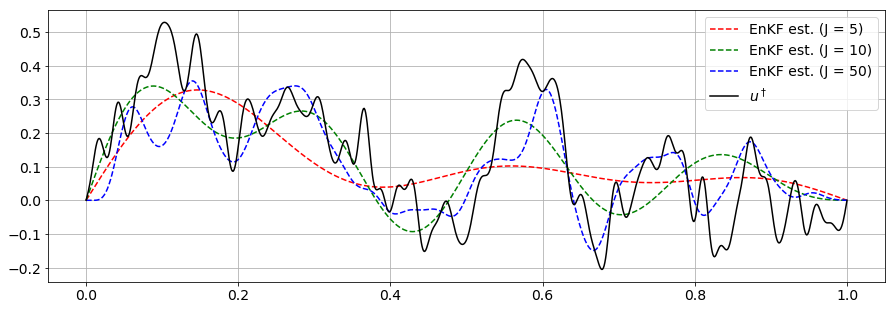
\includegraphics[scale=0.35]{multi_plot.png}
    \caption{Comparison of the truth to several EnKF estimates for $J = 5, 10, 50$}
\end{figure}

\begin{figure} \label{fig-2}
    \centering
    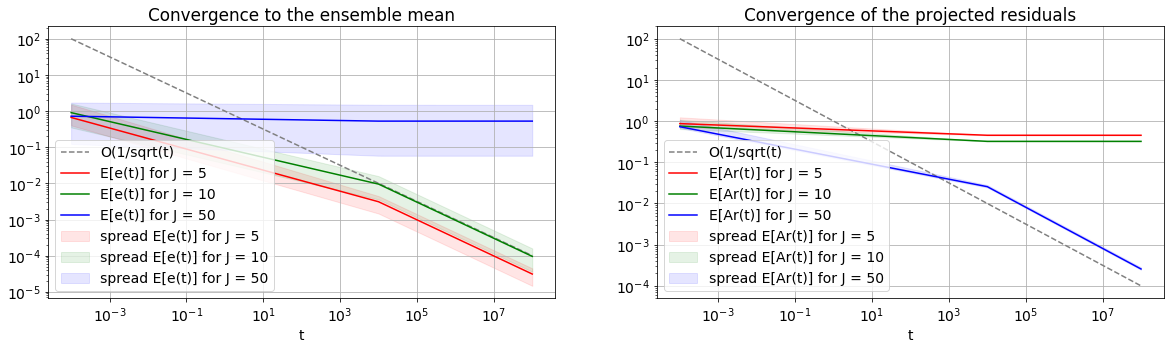
\includegraphics[scale=0.30]{convergence_plot.png}
    \caption{Convergence of EnKF the estimates for $J = 5, 10, 50$}
\end{figure}

We now wish to observe the convergence properties of the continuous-time limite of the EnKF algorithm. Since
the Gaussian process system is not finite dimensional, a discretization is required. We base
this discretization on a spectral Karhunen–Loève expansion of the Gaussian process which is 
then cut to a finite number of terms, $N = 100$.

In the algorothm, the initial ensemble is constructed based on the 
first $J$ eigenpairs $(\lambda_j, \psi_j)$ of the KL expansion. Thus
$u^{(j)} = \sqrt{\lambda_j}\psi_j z_j$ where $\{z_j\}_{j=1} ^J$ are i.i.d.
realizations of $\text{N}(0, 1)$ and
\begin{equation*}
    \lambda_j = (\pi j)^{-2} \qquad \psi_j(x) = \sqrt{2}\sin(\pi n x).
\end{equation*}

Results of the experiments are to be found in figures \ref{fig-1} and \ref{fig-2}.

\bibliographystyle{abbrv}
\bibliography{../literature/literature.bib}

\end{document}
